% Generated by documents/paper/figures/make_rq_appendix.py from the rq02_da_vs_train_tokens README; do not edit.
\clearpage
\section{Decision accuracy against the tokens of the language seen}
\label{app:rq02_da_vs_train_tokens}

\paragraph{Question.} Does a language's BPB rank the design variants like the reference once the proxy has seen enough of that language?

\paragraph{Setup.} The bits per byte of 50 languages, one task each; design pairs among the variants that train the language (at least three per language), every data build at seed 1904, proxies 90M--1B and the 1.7B run's own early checkpoints. A point is the mean over languages of DA-goal (a checkpoint against the 1.7B final) at one size and tenth of the run, placed at the tokens of the language seen.

\paragraph{Key finding.} \textbf{The 600M rung is the outlier, not the smallest proxy.} At the final checkpoint DA-goal is 0.96 at 90M and 175M, 0.92 at 350M, 0.74 at 600M and 0.92 at 1B (standard error over languages 0.006--0.010). (Figure~\ref{fig:app_rq02_da_vs_train_tokens}.)

\begin{figure}[h]
\centering
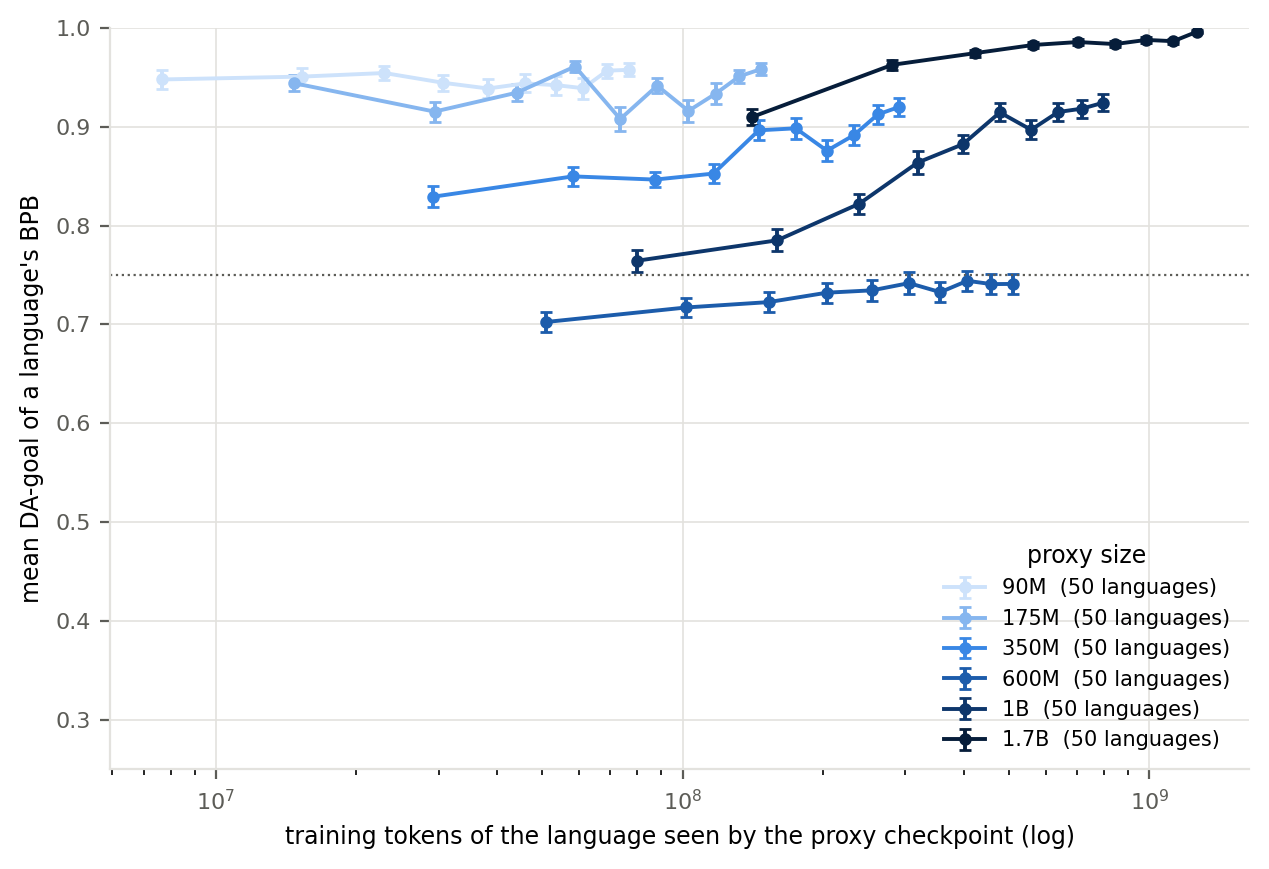
\includegraphics[width=\textwidth]{figures/app_da_goal_multi_axes_bpb.png}
% source: src/signal-and-noise/analysis/rq02_da_vs_train_tokens/pretraining/predictivity_seeds/da_goal_multi_axes_across_langs_bpb_paper.png
\caption{DA-goal of BPB vs tokens seen.}
\label{fig:app_rq02_da_vs_train_tokens}
\end{figure}
